\subsection{x86}

\subsubsection{MSVC}

\IFRU{Имеем в итоге}{What we have after compilation} (MSVC 2010 Express):

\lstinputlisting[caption=MSVC 2010 Express]{patterns/05_passing_arguments/msvc.asm}

\index{x86!\Registers!EBP}
\IFRU{Итак, здесь видно: в функции \main заталкиваются три числа в стек и вызывается 
функция \TT{f(int,int,int)}.}
{What we see is the 3 numbers are pushing to stack in function \main and \TT{f(int,int,int)} 
is called then.}
\IFRU{Внутри \TT{f()}, доступ к аргументам, также как и к локальным переменным, происходит через макросы: 
\TT{\_a\$ = 8}, но разница в том, что эти смещения со знаком \IT{плюс}, 
таким образом если прибавить макрос \TT{\_a\$} к указателю на \EBP, то адресуется \IT{внешняя} 
часть \glslink{stack frame}{фрейма} стека относительно \EBP.}
{Argument access inside \TT{f()} is organized with the help of macros like: \TT{\_a\$ = 8}, 
in the same way as local variables accessed,
but the difference in that these offsets are positive 
(addressed with \IT{plus} sign).
So, adding \TT{\_a\$} macro to the value in the \EBP register, \IT{outer} side of \gls{stack frame} is addressed.}

\index{x86!\Instructions!IMUL}
\index{x86!\Instructions!ADD}
\IFRU{Далее все более-менее просто: значение a помещается в \EAX. 
Далее \EAX умножается при помощи инструкции \IMUL на то что лежит в \TT{\_b}, 
так в \EAX остается произведение\FNPRODUCT этих двух значений.}
{Then \TT{a} value is stored into \EAX. After \IMUL instruction execution, value in the \EAX is 
a product\FNPRODUCT of value in \EAX and what is stored in \TT{\_b}.}
\IFRU{Далее к регистру \EAX прибавляется то что лежит в \TT{\_c}.}
{After \IMUL execution, \ADD is 
summing value in \EAX and what is stored in \TT{\_c}.}
\IFRU{Значение из \EAX никуда не нужно перекладывать, оно уже лежит где надо. 
Возвращаем управление вызываемой 
функции ~--- она возьмет значение из \EAX и отправит его в \printf.}
{Value in the \EAX is not needed to be moved: it is already in place it must be.
Now return to \gls{caller}~---it will take value from the \EAX and used it as \printf argument.}

\subsubsection{MSVC + \olly}

\IFRU{Проиллюстрируем всё это в}{Let's illustrate this in} \olly.
\IFRU{Когда мы протрассируем до первой инструкции в \TT{f()}, которая использует какой-то из аргументов
(первый), мы увидим что \EBP указывает на \glslink{stack frame}{фрейм стека}, 
я отметил его начало красной стрелкой}{When 
we trace until the very first instruction in \TT{f()} that uses one of the arguments (first one),
we see that \EBP is pointing to the \gls{stack frame}, I marked its begin with red arrow}.
\IFRU{Самый первый элемент \glslink{stack frame}{фрейма стека} это сохраненное значение \EBP, 
затем \ac{RA}, третий элемент это
первый аргумент ф-ции, затем второй аргумент и третий}{The first element of \gls{stack frame} is saved \EBP value, 
second is \ac{RA}, third is first function argument, then second argument and third one}.
\IFRU{Для доступа к первому аргументу ф-ции, нужно прибавить к \EBP аккурат 8 (2 32-битных слова)}
{To access the first function argument, one need to add exactly 8 (2 32-bit words) to \EBP}.

\begin{figure}[H]
\centering
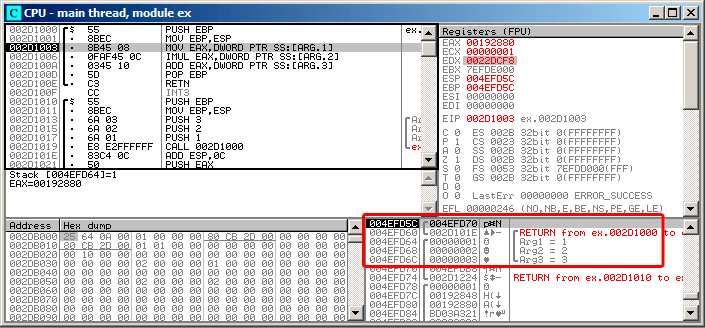
\includegraphics[scale=0.66]{patterns/05_passing_arguments/olly.png}
\caption{\olly: \IFRU{внутри ф-ции}{inside of} f()\EN{ function}}
\label{fig:passing_arguments_olly}
\end{figure}

\subsubsection{GCC}

\IFRU{Скомпилируем то же в GCC 4.4.1 и посмотрим результат в \IDA:}
{Let's compile the same in GCC 4.4.1 and let's see results in \IDA:}

\lstinputlisting[caption=GCC 4.4.1]{patterns/05_passing_arguments/gcc.asm}

\IFRU{Практически то же самое, если не считать мелких отличий описанных раннее.}
{Almost the same result.}

\IFRU{После вызова обоих ф-ций, \glslink{stack pointer}{указатель стека} не возвращается назад, потому что предпоследняя
инструкция}{The \gls{stack pointer} is not returning back after both function exeuction, because penultimate}
\TT{LEAVE} (\ref{x86_ins:LEAVE}) \IFRU{сделает это за один раз, в конце исполнения}{instruction will do this,
at the end}.

